\documentclass[12pt,a4paper]{report}
\usepackage[utf8]{inputenc}
\usepackage{amsmath}
\usepackage{amsfonts}
\usepackage{amssymb}
\usepackage{graphicx}
\usepackage{enumitem}
\usepackage[left=2cm, right=2cm, top=4cm, bottom=2cm]{geometry}

\begin{document}
	\begin{titlepage}
		\centering
		{\scshape\LARGE Universidad Nacional Autónoma de México \par}
		\vspace{1cm}
		{\scshape\Large Probabilidad I\par}
		\vspace{1.5cm}
		{\huge\bfseries Tarea IV\par}
		\vspace{.5cm}
		
		{\Large\itshape Alan Ernesto Arteaga Vázquez \par}
		 \vspace{.5cm}
		{\Large\itshape Raúl Llamosas Alvarado \par}
		 \vspace{.5cm}
		{\Large\itshape Edgar Quiroz Castañeda \par}
	    \vspace{.5cm}
		{\Large\itshape Jean Paul Ruiz Melo\par}
		\vspace{.5cm}
		{\Large\itshape Sandra Del Mar Soto Corderi \par}
		
		\vfill
		 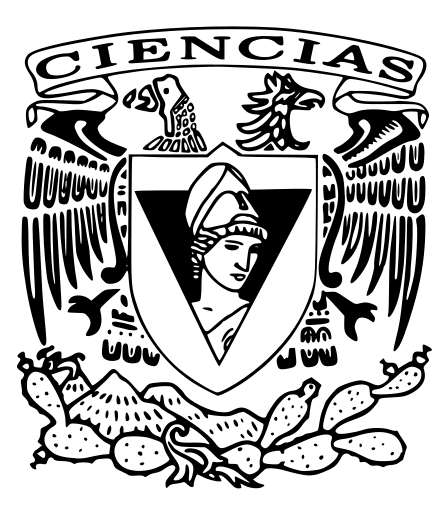
\includegraphics[width=0.5\textwidth]{escudo.png}
		\vfill

		{\large Lunes 15 de octubre del 2018 \par}
	\end{titlepage}

	\pagebreak
	\setlength{\voffset}{-0.75in}
	\setlength{\headsep}{5pt}

	\begin{enumerate}
		\item {
			Sea $A$ un evento $(A \in F)$. Definimos $X$ por
			\[
				X(\omega) =
				\begin{cases}
					1, $ si $\omega \in A\\
					0, $ si $\omega \not\in A
				\end{cases}
			\]
			¿Es $X$ variable aleatoria?
		}
		\item {
			Considere un espacio de probabilidad $\Omega = \{1, 2, 3, 4, 5, 6\}$ y
			$F = \{\emptyset, \Omega, \{2, 4, 6\}, \{1, 3, 4\}\}$.\\
			Sean $X_1, X_2 : \Omega \rightarrow \mathbb{R}$ definidas como
			\begin{align*}
				X_1(\omega) = \omega^2 & X_2(\omega) = \begin{cases}
																								1, \omega $ par$\\
																								0, \omega $ impar$
																							\end{cases}
			\end{align*}
			¿Son $X_1$ y $X_2$ variables aleatorias en este espacio de probabilidad?
		}
		\item {
			Sea $f$ una función definida por
			\[
				f(x) = \begin{cases}
								x+1, $ si $ -1 \leq x \leq 0\\
								2x-6, $ si $ 3 \leq x \leq c\\
								0, $ en otro caso$
			\end{cases}
			\]
			Con $c$ constante.
			\begin{enumerate}
				\item {
					Determine el valor de $c$ de tal manera que $f$ sea una función de
					densidad.
				}
				\item {
					Encuentre la función de distribución correspondiente a $f$.
				}
			\end{enumerate}
		}
		\item {
			Sea $f$ una función definida por
			\[
				f(x) = \begin{cases}
								cr^x, $ si $ x \in \{0, 1, ...\}\\
								0, $ en otro caso$
							 \end{cases}
			\]
			En donde $0 < r < 1$. Encuentre $c$ para que $f$ sea función de densidad.
		}
		\item {
		La función de densidad de una variable aleatoria $X$ es
		\[f_X(x) = \gamma x^2 e^{-kx}\mathbb{I}_{(0, \infty)}\]
		Donde $k > 0$.
		\begin{enumerate}
			\item {
				Encontrar el valor de $\gamma$.
			}
			\item {
				Encontrar la función de distribución $F_X$ de la variable aleatoria
				$X$.
			}
			\item {
				Calcule $P(0 < X < \frac{1}{k})$
			}
		\end{enumerate}
		}
		\item {
			Sea
			\[
				f(x) = \begin{cases}
								0, $ si $ x < 0\\
								\frac{1}{2}\beta, $ si $ 0 \leq x < 1\\
								\frac{1}{2}, $ si $ 1 \leq x < 2\\
								\frac{1}{2}(1-\beta), $ si $ 2 < x < 3\\
								0, $ si $ x \geq 3
						 	 \end{cases}
			\]
			Donde $0 < \beta < 1$. Encontrar la función de distribución $F_X$
		}
		\item {
			Demuestre que $f_X(x) = \frac{1}{2}e^{-|x|}\mathbb{I}_\mathbb{R}(x)$ es
			una función de densidad.
		}
		\item {
			Sea $X$ una variable aleatoria con función de densidad
				\[f_\gamma(y) = cy \mathbb{I}_{\{1, 2, 3, 4\}}(y)\]
				\begin{enumerate}
					\item {
						Determinar el valir de $c$ para que $f_\gamma$ sea una función de
						densidad de probabilidad.
					}
					\item {
						Calcule $P(1 < Y \leq 3)$ y $p(Y < 1 | Y \leq 3)$
					}
				\end{enumerate}
		}
		\item {
			Sea $X$ una variable aleatoria continua con función de densidad
				\[
					f_X(x) = \begin{cases}
										6x(1-x), $ si $ 0 < x < 1\\
										0, $ en otro caso$
									 \end{cases}
				\]
			Calcule $P(|X-\frac{1}{2}| > \frac{1}{4})$.
		}
		\item {
			Suponga que se selecciona aleatoriamente un punto $z$ del cuadrado con
			esquinas (2, 1), (3, 1), (2, 2,) y (3, 2). Sea $A$ la variable aleatoria
			que mide el área del triángulo con vértices (2, 1), (3, 1) y $z$.
			\begin{enumerate}
				\item {
					¿Cuál es el valor más grande que $A$ puede tomar?
				}
				\item {
					¿Cuál es el conjunto de puntos para el cuál $A \leq \frac{1}{2}$?
				}
				\item {
					Encuentre la función de densidad de $A$.
				}
				\item {
					Encuentre la función de distribución de $A$.
				}
			\end{enumerate}
		}
		\item {
			Una póliza de seguros cubre las reclamaciones médicas de los empleados
			de una pequeña compañía.\\
			El valor $V$ de las reclamaciones hechas en un año es descrita mediante
			\[V = 100000Y\]
			Donde $Y$ es una variable aleatoria con función de densidad
			\[
				f_\gamma(y) = \begin{cases}
												k(1-y)^4, $ si $ 0 < y < 1\\
												0, $ en otro caso$
											\end{cases}
			\]
			Donde $k$ es constante. ¿Cuál es la probabilidad de que $V$ exceda 10000?
			}
		\item {
			Una urna contiene 5 bolas rojas y 5 bolas azules. Se realiza un juego
			que consiste en extraer aleatoriamente 2 bolas de la urna. Suponga que
			si se extraen dos bolas del mismo color, el jugador gana \$1.11 y si se
			extraen dos bolas de distinto color el jugador pierde \$1.00. Si una
			persona participa en el juego dos veces, calcule la probabilidad de que
			la ganancia de esta persona sea mayos a \$0.00.
		}
		\item {
			Sea $X$ una variable aleatoria con función de densidad dada por
			\[f_X(x) = \frac{1}{1}e^{-|x|}\mathbb{I}_{\mathbb{R}}(x)\]
			Si $Y = X^2$, encuentre la función de distribución acumulada de $Y$.
		}
		\item {
			Sea $X$ una variable aleatoria con función de densidad dada por
			\[
				f_X(x) = \begin{cases}
									4x^3, $ si $ 0 < x < 1\\
									0, $ en otro caso$
								 \end{cases}
			\]
			Encuentre $P(X \leq \frac{2}{3}|X > \frac{1}{3})$.
		}
	\end{enumerate}
\end{document}
